\section{Best Practices}

In the author's personal experience, there is often a certain opacity in the projection-based ROM literature on the subject of data preparation and robustness controls. In many cases this is simply due to the fact that many ROM studies deal with systems which are governed by a single state variable (Burgers' equation, Kuramoto--Sivashinsky equation), are governed by state variables that are naturally of similar magnitudes (shallow water equations, Euler equations for Sod shock tube), or are commonly non-dimensionalized in open-source or commercial solvers (incompressible Navier--Stokes). In such situations, the dimensionality of the state variables is either irrelevant or has little effect on the accuracy of state representations and the solution of the ROM equations. Sometimes, however, small but crucial details of data preparation or the ROM solution are left out as they are considered self-evident to the authors (as has been discovered anecdotally by this author and colleagues). To date, the work by Parish and Rizzi~\cite{Parish2022} provides the most explicit description and comprehensive study of ensuring a dimensionally-consistent POD formulation and ROM solution by careful choice of inner products. Although the focus of their work is the compressible Euler equations, they provides broadly-meaningful insights for dimensional dynamical systems.

All but one numerical experiment in this thesis deals with high-pressure, compressible reacting flows, which are characterized by both vastly disparate magnitudes in the system state and an inability to readily non-dimensionalize the governing equations. As such, careful data preparation and unsteady solution robustness controls are extremely important in enabling the stable and accurate solution of projection-based reduced-order models. Further, we wish to be as transparent about every element of the ROM construction process to help enable successful ROMs for future researchers working with similarly-complex systems. We detail some of the key elements in this process that are explored in the numerical experiments which follow.

\subsection{Centering and Scaling}\label{subsec:centerScale}
%
As previously defined, the general (linear or non-linear) low-dimensional state representation for the conserved and target states are defined, respectively, as
%
\begin{align}
	\consVecRom &\defEq \consVecCent + \consScale \nnLayer_{\decoderVar,\consVar}\left(\consVecCoef\right), \\
	\primVecRom &\defEq \primVecCent + \primScale \nnLayer_{\decoderVar,\primVar} \left(\primVecCoef\right),
\end{align}
%
where, again, the functions $\nnLayer_{\decoderVar,\consVar}\left(\consVecCoef\right) = \consTrial \consVecCoef$ and $\nnLayer_{\decoderVar,\primVar}\left(\primVecCoef\right) = \primTrial \primVecCoef$ for a linear trial space. This decomposition by centering ($\consVecCent$, $\primVecCent$) and the scaling ($\consScale$, $\primScale$) operation is often referred to as \textit{feature scaling} in the machine learning community, whereby the training datasets are constructed (as noted in Eqs~\ref{eq:consSnapMat} and~\ref{eq:primSnapMat}) by
%
\begin{align}
	\consDataMatUns &= \left[ \consScaleInv\left[\consFunc{\initTime} - \consVecCent\right], \; \hdots \; , \; \consScaleInv\left[\consFunc{\finalTime} - \consVecCent \right] \right], \\
	\primDataMatUns &= \left[ \primScaleInv\left[\primFunc{\initTime} - \consVecCent\right], \; \hdots \; , \; \primScaleInv\left[\primFunc{\finalTime} - \primVecCent \right] \right].
\end{align}
%
The choice of $\consVecCent$/$\consScale$ and $\primVecCent$/$\primScale$ has a measurable influence on the accuracy of the above approximations, particularly for variables of extremely disparate magnitudes. Before demonstrating this fact, we outline and compare several popular methods of centering and scaling.

\paragraph*{Centering}\mbox{}\\
%
With the exception of centering for min-max scaling, all centering methods described here are considered to be spatially-variant, i.e. $\consVecCent \defEq \consVecCent(\spatialVec)$, $\primVecCent \defEq \primVecCent(\spatialVec)$. We describe each in turn.

\begin{enumerate}
	\item \textit{Initial condition}: Centering about the initial condition, i.e. $\consVecCent = \consVec(\initTime)$ or $\primVecCent = \primVec(\initTime)$, results in approximation of the unsteady state as perturbations about the initial condition. In the case of a linear trial space, this guarantees exact satisfaction of the initial conditions, as the projection of the zero vector (the initial condition subtracted by itself) is identically zero. In the case of autoencoder non-linear manifold methods, however, this is merely satisfied approximately, and near-satisfaction is encouraged by including the zero vector in the training set and initializing the non-linear manifold ROM from the encoding of the zero vector, as in~\cite{Lee2020}.

	\item \textit{Mean}: The mean field centering computes the centering vector as the arithmetic mean of the data snapshots,
	%
	\begin{align}
		\consVecCent &= \frac{1}{\numSnaps} \sum_{\timeIdx=1}^{\numSnaps} \consVec^{\timeIdx} \label{eq:meanCentCons}\\
		\primVecCent &= \frac{1}{\numSnaps} \sum_{\timeIdx=1}^{\numSnaps} \primVec^{\timeIdx} \label{eq:meanCentPrim}
	\end{align}
	%
	This concept is fairly common in the turbulence modeling community, which often seeks to accurately describe unsteady perturbations about the time-averaged field for statistically-stationary flows. In the same sense, centering data snapshots about the mean field ensures that the low-dimensional representation accurately captures these small-scale fluctuations which would otherwise be dwarfed by the mean field.

	\item \textit{Min-max}: Min-max feature scaling, composed of associated centering and scaling operations (see below for the scaling operation), has the effect of ensuring that all values in the modified dataset fall in the range $[0.0, \; 1.0]$. For the $\varIdx$th state variable (e.g. density, velocity), the centering vector is computed as
	%
	\begin{align}
		\consValCentVar &= min\left(\consDataMatVar\right), \quad \consVecCentVar\left(\spatialVec_{\dummyIdx}\right) = \consValCentVar \; \forall \; \dummyIdx \in \{1, \; \hdots, \; \numCells\} \\
		\primValCentVar &= min\left(\primDataMatVar\right), \quad \primVecCentVar\left(\spatialVec_{\dummyIdx}\right) = \primValCentVar \; \forall \; \dummyIdx \in \{1, \; \hdots, \; \numCells\}
	\end{align}
	%
	where the data snapshot matrix for the $\varIdx$th state variable is given by
	%
	\begin{align}
		\consDataMatVar &\defEq \left[ \consVecVar\left(\initTime\right), \; \hdots, \; \consVecVar\left(\finalTime\right) \right] \label{eq:consDataMat}\\
		\primDataMatVar &\defEq \left[ \primVecVar\left(\initTime\right), \; \hdots, \; \primVecVar\left(\finalTime\right) \right] \label{eq:primDataMat}
	\end{align}
	%
	We direct the reader to the min-max scaling description below for further details on this approach.
\end{enumerate}

\paragraph*{Scaling}\mbox{}\\
%
For all methods described below, the scaling matrices $\consScale$, $\primScale$ are composed of constant scalars which are specific to a given state variable (e.g., density, velocity) but are not specific to spatial location. This can be written as as
%
\begin{align}
	\consScale &\defEq diag\left(\consScaleVecVar{1}^\top, \; \hdots, \; \consScaleVecVar{\numVars}^\top \right), \quad \consScaleVecVar{\varIdx}\left(\spatialVec_{\dummyIdx}\right) = \consScaleVar{\varIdx} \; \forall \; \dummyIdx \in \{1, \; \hdots, \; \numCells\} \\
	\primScale &\defEq diag\left(\primScaleVecVar{1}^\top, \; \hdots, \; \primScaleVecVar{\numVars}^\top \right), \quad \primScaleVecVar{\varIdx}\left(\spatialVec_{\dummyIdx}\right) = \primScaleVar{\varIdx} \; \forall \; \dummyIdx \in \{1, \; \hdots, \; \numCells\}
\end{align}
%
where $\consScaleVecVar{\varIdx}$, $\primScaleVecVar{\varIdx} \in \mathbb{R}$ is the constant conservative/target scaling value for the $\varIdx$ state variable.

\begin{enumerate}
	\item $\ell^2$-norm: Scaling by the $\ell^2$-norm method is motivated by that proposed by Lumley and Poje~\cite{Lumley1997}, and is computed as
	%
	\begin{align}
		\consScaleVar{\varIdx} &= \frac{1}{\numSnaps} \sum_{\timeIdx=1}^{\numSnaps} \left\Vert \consVecVar^{\timeIdx} - \consVecCentVar \right\Vert^2 \\
		\primScaleVar{\varIdx} &= \frac{1}{\numSnaps} \sum_{\timeIdx=1}^{\numSnaps} \left\Vert \primVecVar^{\timeIdx} - \primVecCentVar \right\Vert^2
	\end{align}
	This has the effect of ensuring that all state variable vectors have an length (in the Euclidean norm) close to unity. This is closely related to the POD, which computes the distance between the data and its projection in the $\ell^2$ norm.

	\item Standardization: Data standardization is coupled with the calculation of the mean field, as described above. The scaling constants are calculated as
	%
	\begin{align}
		\consScaleVar{\varIdx} &= \sqrt{\frac{1}{\numSnaps \numCells} \sum_{\timeIdx=1}^{\numSnaps} \sum_{\dummyIdx = 1}^{\numCells} \left[\consVecVar^{\timeIdx}\left(\spatialVec_{\dummyIdx}\right) - \consVecCentVar\left(\spatialVec_{\dummyIdx}\right) \right]^2} \\
		\primScaleVar{\varIdx} &= \sqrt{\frac{1}{\numSnaps \numCells} \sum_{\timeIdx=1}^{\numSnaps} \sum_{\dummyIdx = 1}^{\numCells} \left[\primVecVar^{\timeIdx}\left(\spatialVec_{\dummyIdx}\right) - \primVecCentVar\left(\spatialVec_{\dummyIdx}\right) \right]^2}
	\end{align}
	%
	which is the standard deviation for the $\varIdx$th state variable of the dataset and $\consVecCentVar$, $\primVecCentVar$ are the mean field for the $\varIdx$th state variable as calculated in Eq.~\ref{eq:meanCentCons} and~\ref{eq:meanCentPrim}. This operation has the effect of ensuring that the centered and scaled dataset for each state variable has a mean of zero and standard deviation of one.

	\item Min-max: As stated for the min-max centering above, the min-max scaling and centering are strictly coupled, and the implementation of both results in scaling all variables such that they fall within the range $[0.0, \; 1.0]$. The scaling values are computed as
	%
	\begin{align}
		\consScaleVar{\varIdx} &= max\left(\consDataMatVar\right) - min\left(\consDataMatVar\right) \\
		\primScaleVar{\varIdx} &= max\left(\primDataMatVar\right) - min\left(\primDataMatVar\right)
	\end{align}
	%
	where the data matrices are given as in Eqs.~\ref{eq:consDataMat} and~\ref{eq:primDataMat}.

	Although min-max scaling is fairly common within the machine learning community, and is a simple method of ensuring that the data are roughly the same order of magnitude, this scaling has the effect of emphasizing outliers, which thus define the maximum and minimum bounds of the state variables.
\end{enumerate}

\subsection{Residual Weighting}\label{subsec:resWeight}

\subsection{Limiters}

\subsection{POD Energy}

For a linear representation computed by POD, choosing the dimension of the trial bases $\consTrial$ or $\primTrial$, and the dimension of the gappy POD regression basis for hyper-reduction $\deimBasis$, is not an exact science. Although a given POD basis is $\ell^2$-optimal for a given dimension $\numConsModes$, $\numPrimModes$, or $\numResModes$, it is impossible to know \textit{a priori} how the accuracy of the representation will affect the unsteady solution of a PROM for a general non-linear system. In fact, enrichment of the trial space by increasing the basis dimension is never guaranteed to improve PROM accuracy. Numerical experiments have shown that increasing the trial space dimension may even lead to numerical instabilities~\cite{Huang2022}.

Despite this problem, one must use some heuristics for initial experimentation with projection based ROMs, as computing a uniform grid search over the trial space dimension can be cost-prohibitive, especially for large-scale systems. By far the most popular heuristic is the \textit{POD energy}, or conversely the POD residual energy (unity minus the POD energy). The latter measure is often reported as a percentage, given by the calculation
%
\begin{equation}\label{eq:podEnergyResidual}
    \text{POD Residual Energy}, \% = 100 \times \left( 1 - \frac{\sum_{\dummyIdx=1}^{\numConsModes} \singVal_{\dummyIdx}^2}{\sum_{\dummyIdx=1}^{\numSnaps} \singVal_{\dummyIdx}^2} \right).
\end{equation}
%
where $\singVal_{\dummyIdx} \in \nonnegReals$ are the singular values of the training dataset, computed by the SVD and ordered such that $\singVal_1 \ge \singVal_2 \ge \hdots \ge \singVal_{\numConsModes} \ge 0$.

This measure dates back to the origins of POD, when it was used to decompose and analyze turbulent velocity fields~\cite{berkoozPOD}.
In that context, the POD energy is an analogue of the kinetic energy contributed by a given trial mode, with lower mode numbers (associated with low-frequency, high-amplitude waveforms) contributing a relatively large portion of the energy, while the high mode numbers (associated with high-frequency, low-amplitude waveforms) contributing relatively little. The extension of POD energy to general flow fields does not always have quite a clear relationship, but helps form a good first guess for how well the trial basis will represent the unsteady flow field.

Projection-based ROM practitioners will generally begin experimentation with trial bases achieving a POD residual energy of approximately 1.0\%, 0.1\%, and 0.01\%. Figure~\ref{fig:samplePODEnergy} displays a sample POD residual energy decay for the two-dimensional transonic cavity flow presented in Chapter~\ref{chap:CavityAndCVRC} for datasets spanning different simulation periods. For the 6 ms case, then, the practitioner might initially experiment with trial bases composed of the leading 19, 64, and 121 modes, corresponding to 1.0\%, 0.1\%, and 0.01\% residual energy.

\begin{figure}
	\centering
	\includegraphics[width=0.6\linewidth]{example-image-a}
	% 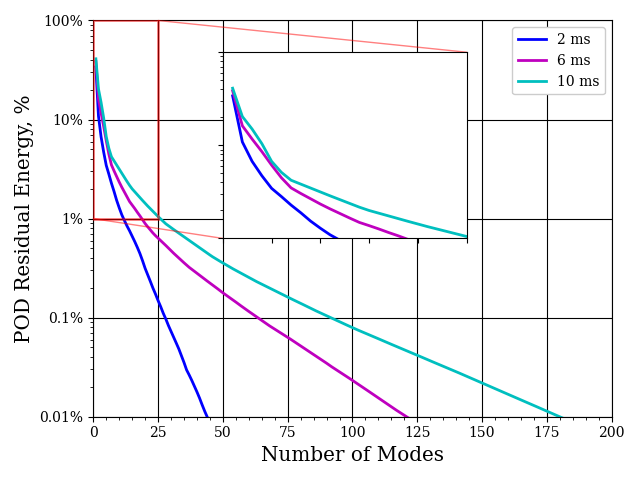
\includegraphics[width=0.6\linewidth]{Chapters/ProjROMs/Images/pod_energy_2dCavity_example.png}
	\caption{\label{fig:samplePODEnergy}Example of POD residual energy decay for 2D cavity case, for datasets encompassing 2, 6, and 10 milliseconds of simulation time.}
\end{figure}

Such explorations of POD residual energy for datasets of varying sizes have the additional benefit of indicating whether a dataset describes a statistically-stationary flow. That is, when adding additional snapshots to the dataset does not result in a significant change in its spectral content, the dataset can be considered to capture the characteristic physics of the system. As can be seen in Fig.~\ref{fig:samplePODEnergy}, while it appears that the lower-frequency ($< 25$ modes) has somewhat converged, there is no indication that the higher-frequency spectral content has converged.

\subsection{Projection Error}\label{subsec:projError}

For results presented in Chapters~\ref{chap:CavityAndCVRC}-\ref{chap:TransientFlame}, we will make frequent use of the \textit{projection error} as a diagnostic tool for understanding the quality of a computed trial manifold $\trialSpace$ in modeling the FOM solution data. This error measure, with a linear trial space for the $\timeIdx$th time instance of the $\varIdx$th state variable (density, $x$-momentum, etc.), is given by the formulation
%
\begin{equation}\label{eq:projErrLinear}
    \errVecVar^\timeIdx = \frac{\left\Vert \stateVecVar^\timeIdx - \left[\stateVecCent + \scaleMat \basisMat \basisMat^\top \scaleMatInv \left[ \stateVecVar^\timeIdx - \stateVecCent \right] \right] \right\Vert_2}{\left\Vert \stateVecVar^\timeIdx \right\Vert_2}.
\end{equation}
%
Scaling the error for each variable by the norm of the unprojected state ensures reasonable comparisons of error between state variables of drastically different magnitudes (e.g., $\bigO{1\text{e}6}$ for pressure and $\bigO{1}$ for species mass fractions). For a non-linear trial manifold $\trialSpace$, an equivalent projection operation akin to $\basisMat \basisMat^\top$ does not exist. Instead, the projection error is defined as
%
\begin{equation}\label{eq:projErrNonlin}
    \errVecVar^\timeIdx = \frac{\left\Vert \stateVecVar^\timeIdx - \argmin{\dummyVec \in \trialSpace} \left\Vert \stateVecVar^\timeIdx - \dummyVec \right\Vert_2 \right\Vert_2}{\left\Vert \stateVecVar^\timeIdx \right\Vert_2}.
\end{equation}
%
As $\trialSpace$ is a non-linear manifold defined by the range of the decoder $\decoderFunc{\cdot}$, the solution of the $argmin$ is a non-linear least squares problem. In practice, we use the \verb|optimize.least_squares()| function provided by the SciPy Python package (with default tolerances) to compute this solution. An initial guess for the input to the decoder is given by the encoding of the state, $\encoderFunc{\stateVec^{\timeIdx}}$. This process effectively finds the point on the non-linear trial manifold which is closest to the data $\stateVec^{\timeIdx}$.

Often the time average over the simulation period $[\initTime, \finalTime]$ will be provided, and is computed as
%
\begin{equation}
    \errVecVar = \frac{1}{\numSnaps} \sum_{\timeIdx = 1}^{\numSnaps} \errVecVar^\timeIdx.
\end{equation}
%
Further, the total average projection error across all state variables provides a very broad measure of the trial space quality, and is given by
%
\begin{equation}
    \errVec = \frac{1}{\numVars} \sum_{\varIdx = 1}^{\numVars} \errVecVar.
\end{equation}
%
Examples of these error measures are provided for a one-dimensional transient flame simulation, similar to those detailed in Chapter~\ref{chap:TransientFlame}, though without acoustic forcing at the outlet. Figures~\ref{fig:projErrTempField} and~\ref{fig:projErrMFField} display instantaneous snapshots of temperature and reactant mass fraction fields, respectively, and the corresponding projections onto a linear trial space and non-linear manifold (by deep convolutional autoencoder) of dimension $\numPrimModes = 3$. Figures~\ref{fig:projErrTempTime} and~\ref{fig:projErrMFTime} display the $\ell^2$ error measure over time, as described by Eqs.~\ref{eq:projErrLinear} and~\ref{eq:projErrNonlin}.
%
\begin{figure}
    \begin{minipage}{0.45\linewidth}
        \includegraphics[width=0.99\linewidth]{example-image-a}
		% 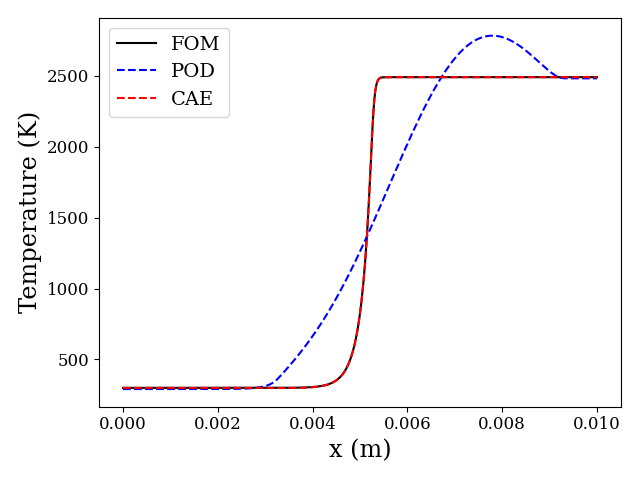
\includegraphics[width=0.99\linewidth]{/home/chris/Research/thesis_data/1d_flame/proj_err_method/temp_proj_field.png}
        \caption{\label{fig:projErrTempField}Instantaneous temperature fields and projections, $\numPrimModes = 3$.}
    \end{minipage}
    \hspace{1em}
    \begin{minipage}{0.45\linewidth}
        \includegraphics[width=0.99\linewidth]{example-image-a}
		% 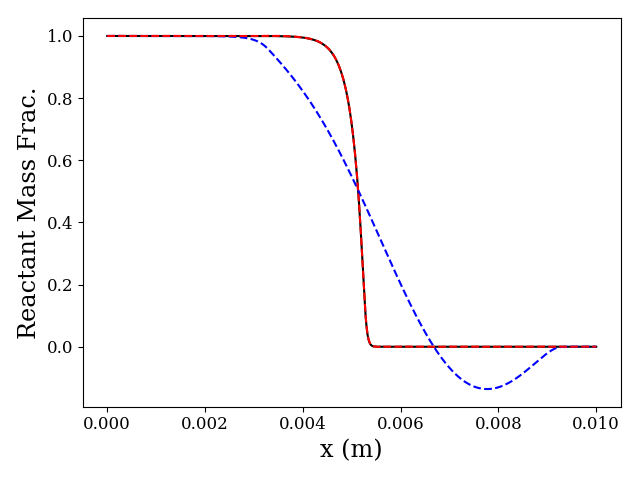
\includegraphics[width=0.99\linewidth]{/home/chris/Research/thesis_data/1d_flame/proj_err_method/mf_proj_field.png}
        \caption{\label{fig:projErrMFField}Instantaneous mass fraction fields and projections, $\numPrimModes = 3$.}
    \end{minipage}
\end{figure}
%
\begin{figure}
    \begin{minipage}{0.45\linewidth}
        \includegraphics[width=0.99\linewidth]{example-image-a}
		% 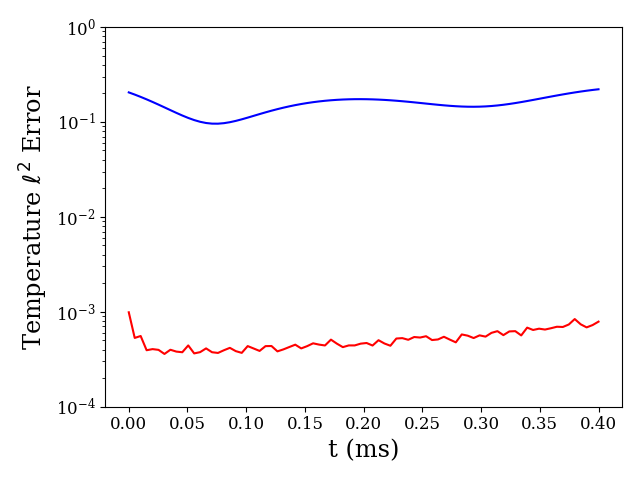
\includegraphics[width=0.99\linewidth]{/home/chris/Research/thesis_data/1d_flame/proj_err_method/temp_error.png}
        \caption{\label{fig:projErrTempTime}Unsteady temperature projection error, $\numPrimModes = 3$.}
    \end{minipage}
    \hspace{1em}
    \begin{minipage}{0.45\linewidth}
        \includegraphics[width=0.99\linewidth]{example-image-a}
		% 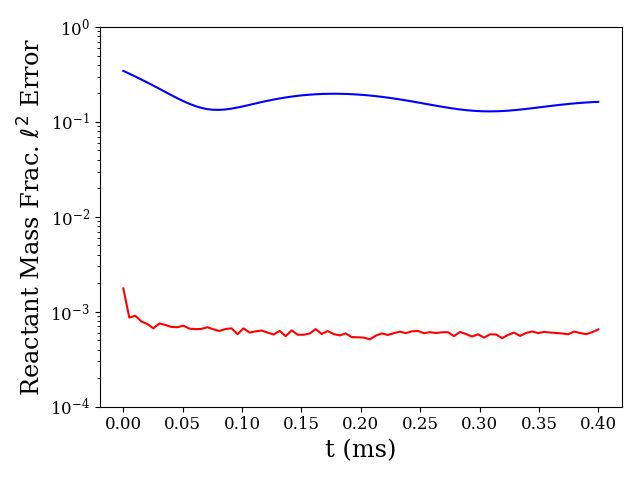
\includegraphics[width=0.99\linewidth]{/home/chris/Research/thesis_data/1d_flame/proj_err_method/mf_error.png}
        \caption{\label{fig:projErrMFTime}Unsteady mass fraction projection error, $\numPrimModes = 3$.}
    \end{minipage}
\end{figure}
%

No analytical \textit{a priori} error measure exists for predicting the error of PROMs of general non-linear systems. Unsteady errors will invariable accumulate and compound over the course of a PROM simulation. However, projection error is useful in providing an upper bound on the accuracy of the PROM. The unsteady PROM cannot produce a solution more accurate that the projected solution (except by pure coincidence), as the trial space is never an exact representation of the true solution. Further, computing the projection of unseen data (in parametric or future state prediction) provides a measure of the generalizability of the trial manifold. This can help determine whether a PROM will be appropriate for such predictions and perhaps preclude expensive online ROMs which are bound to fail purely due to the unfitness of the trial manifold.